\chap{Моделирование и анализ}
	В качестве реализации языка Prolog был выбран SWI-Prolog.
		Это открытая реализация, работающая на Unix, MacOS и Windows.
		В данной реализации имеется необходимы функционал, а именно предикаты nb\_getval, nb\_setval и nb\_current.
		Эти предикаты позволяют использовать другие предикаты в качестве глобальных переменных, что
		позволяет существенно упростить написание правил для вычисления.

	В процессе реализации было создано порядка десяти файлов с описанием правил логического вывода
		общей суммой порядка семиста строк. Такое большое количество правил обусловлено наличием деталей и нюансов.
		Ниже представлен основной файл, в котором реализован инициализация логического вывода.
		Данный код иллюстрирует реализацию формулы времени. Благодаря функционалу SWI-Prolog
		в дальнейшем предикаты отражающие время можно будет указывать в правилах только при необходимости.

	Реализации правил manage\_people и manage\_elevators вынесены в другие файлы,
		как как являются весьма громоздкими.
		Manage\_people отвечает за внешний фактор (случайное появление нуждающихся в лифте людей).
		А manage\_elevators включает в себя формулы движения лифтов.

\section{Пример работы реализации}

	Данный пример иллюстрирует работу группы лифтов, где их количество равно 2, в здании с 5 этажами.
		В ходе работы системы появится два человека в моменты времени $t_2$ и $t_4$ на этажах $e_1$ и $e_0$,
		и у каждого человека целью будет четвёртый этаж $d_4$.

	Изначально первая кабина находится на первом этаже $e_0$, а вторя на втором $e_1$.
		Ниже приведён лог показывающий работу системы:

	Изучив выше изложенный журнал, можно увидеть результат, что каждый человек доставлен и ожидание составило не более одной единицы времени.

\section{SimPy}

SimPy - это Python фреймворк процессо-ориентированной дискретно-событийной системы моделирования. Его диспетчеры событий основаны на функциях-генераторах Python.

Также они могут использоваться для создания асинхронных сетей или для реализации мультиагентных систем (с как моделируемым, так и реальным взаимодействием).

Процессы в SimPy - это просто Python генераторы, которые используются для моделирования активных компонентов, например, таких как покупатели, транспортные средства или агенты. SymPy также обеспечивает различные виды общих ресурсов для моделирования точек с ограниченной пропускной способностью (например, серверов, касс, тоннелей). Начиная с версии 3.1, SimPy также будет обеспечить возможности мониторинга для помощи в сборе статистических данных о ресурсах и процессах. 

SymPy представляет собой открытую библиотеку символьных вычислений на языке Python. Цель SymPy - стать полнофункциональной системой компьютерной алгебры (CAS), при этом сохраняя код максимально понятным и легко расширяемым. SymPy полностью написан на Python и не требует сторонних библиотек.

SymPy можно использовать не только как модуль, но и как отдельную программу. Программа удобна для экспериментов или для обучения. Она использует стандартный терминал IPython, но с уже включенными в нее важными модулями SymPy и определенными переменными x, y, z.

\subsection{Реализация на SimPy}

	Данная симуляция системы управления группой лифтов с ограниченным количеством кабин и несколькими людьми,
		которые приходят для попадания с одного этажа на другой.
		В данной системе используется ресурс для моделирования ограниченного количества кабин.
		Он также определяет процесс выбора кабины и перевозку ей человека.

	Когда человек появляется рядом с шахтой лифта, он вызывает первую из свободных кабин.
		Как только он его кабина забирает, время ожидания человека прекращается.
		Он, наконец, добирается до нужного этажа и уходит.

	После старта системы начинается генерация людей, они появляются после случайного интервала времени,
	пока продолжается симуляция.


	При том, что данная программа является многопоточной, стоит отметить тот факт, что здесь используются общие ресурсы.
		Эти ресурсы могут использоваться для ограничения количества процессов, использующих их одновременно.
		Процесс должен запрашивать право использования ресурса. Как только право на использование больше не требуется,
		оно должно быть выпущено. Данная система смоделирована как ресурс с ограниченным количеством кабин.
		Люди прибывают к кнопке вызова кабины и просят выполнить перевозку на другой этаж.
		Если все кабины заняты, человек должен ждать, пока один из пассажиров не закончит поездку и не освободит кабину.

		\subsection{Пример работы реализации}

	Данный пример иллюстрирует работу группы лифтов, где их количество равно 2, в здании с 30 этажами.
		В ходе работы системы появится люди в случайные моменты времени на случайных этажах этажах,
		и у каждого человека целью является добраться на другой этаж.

	Изначально первая кабина находится на первом этаже $e_0$, а вторя на втором $e_1$.
		Ниже приведён лог показывающий работу системы:

	Изучив выше изложенный журнал, можно увидеть, что за время симуляции появилось 4 человека,
		каждый человек доставлен.

\section{Интеллектуальная реализация}

Однако, пусть реализация логического вывода на языке Prolog является целесообразной задачей, но для разделения моделируемой системы на логический блок и блок взаимодействия объектов необходима клиент-сервергая связка. А реализация сервера или клиента на языке Prolog не является его типовой задачей, что и касается реализации графической составляющей системы моделирования.

	Таким образом более целесообразном будет оставить блок взаимодействия объектов реализованными на языку Prolog.
		Более того, правила описанные для модуляции системы будут использованы
		для построения решения логическим блоком.

	Данный код иллюстрирует реализацию формулы реализующие обход возможных вариантов будущего, сбор статистики с каждого варианта и выбор наиболее подходящего варианта будущего по признаку. в данном случае интересующим признаком является среднее ожидание человеком кабины. 

% \input{src/pl_mod_code.tex}

	Благодаря функционалу SWI-Prolog
		предикаты отражающие состояние системы в момент вызова кабины можно будет указывать в правилах только при необходимости.

		\subsection{Пример работы реализации}

	Данный пример иллюстрирует работу группы лифтов, где их количество равно 2, в здании с 5 этажами.
		В ходе работы системы появится два человека в моменты времени $t_2$ и $t_4$ на этажах $e_1$ и $e_0$,
		и у каждого человека целью будет четвёртый этаж $d_4$.

	Изначально первая кабина находится на первом этаже $e_0$, а вторя на втором $e_1$.
		Ниже приведён лог показывающий работу системы:

		%example

Изучив выше изложенный журнал, можно увидеть, что происходит построение дерева формулы и её обход.
	Для того чтобы было нагляднее следует прокомментировать строку лога.

Первые четыре столбца в логе - это реальное время журналирования момента модуляции.
	Следующим столбцом идёт связка двух чисел, первое число - это номер процесса,
	он необходим для идентификации сессии, а второе число показывает момент времени модуляции.
	Ещё одним столбцом является связка строки и числа, число - это так же момент времени в данной ветки формулы,
	А строка отражает индекс чанка формулы в момент вывода, r означает корень выводимой формулы, а дальше серез нижние подчёркивание перечислены индексы кабин, которые участвуют в логическом выводе в данные момент.

	\section{Сравнительный анализ}

	Как было упомянуто выше одним из основных критериев является средняя длительность ожиданий.
		Так же можно сравнить время выполнения модуляции, объём занимаемой памяти и сложность реализации.
		Под сложностью мы будем понимать суммарное количество строк кода каждого из проектов.

	Сравнив были получены следующие данные.

		Среднее время ожидания:
			% \begin{figure}[!htb]
			%         \includegraphics[width=\linewidth]{src/1.png}
			%         \centering
			% \end{figure}

		Реальное время выполнения модуляции:
			% \begin{figure}[!htb]
			%         \includegraphics[width=\linewidth]{src/2.png}
			%         \centering
			% \end{figure}

		Объём и сложность:
			% \begin{figure}[!htb]
			%         \includegraphics[width=\linewidth]{src/3.png}
			%         \centering
			% \end{figure}

		Входе выполнения экспериментов на выполнение модуляций с большими числами не хватило вычислительной мощи
		оборудования для реализаций на Prolog. Что иллюстрирует потребность в ресурсах у данных подходов
		к решению задачи.

		Но не смотря на провал с большими числами. Третья реализация показала себя лучше, чем остальные.


{
\changefontsizes[12pt]{12pt}
\captionsetup{font=large,margin=21pt}

\vspace{14pt}
\begin{longtable}[t]{@{\extracolsep{\fill}}|l|@{\hskip+35pt}p{0.15\textwidth}|@{\hskip+35pt}p{0.15\textwidth}|@{\hskip+35pt}p{0.15\textwidth}|}
% \begin{longtable}[t]{@{\extracolsep{\fill}}|l|@{\hskip-28pt}c|@{\hskip-28pt}c|@{\hskip-28pt}c|}
	\caption{Сравнение по среднему времени ожидания \vspace{-35pt}} \label{projectt1} \\ \hline
			&&&\\[-7pt]
	Способ управления
		& 30 этажей \hspace{14pt}
			& 15 этажей \hspace{14pt}
				& 5 этажей  \hspace{14pt}  \\  \hline
	\endfirsthead
	\caption* {Продолжение таблицы \ref{projectt1}\vspace{-35pt}}\\ \hline
			&&&\\[-7pt]
	Способ управления
		& 30 этажей
			& 15 этажей
			& 5 этажей   \\ \hline \endhead 
			&&&\\[-7pt]
	I тип     &	7.5		&	6	& 2.7	\\ \hline
			&&&\\[-7pt]
	II тип    &	9.6		&	7.1	& 3.2		\\ \hline
\end{longtable}
}

{
\changefontsizes[12pt]{12pt}
\captionsetup{font=large,margin=10mm}

\vspace{14pt}
\begin{longtable}[t]{@{\extracolsep{\fill}}|l|@{\hskip+35pt}p{0.15\textwidth}|@{\hskip+35pt}p{0.15\textwidth}|@{\hskip+35pt}p{0.15\textwidth}|}
	\caption{Сравнение по времени выполнения  \vspace{-35pt}} \label{projectt2} \\ \hline
			&&&\\[-7pt]
	Способ управления
		& 30 этажей \hspace{14pt}
			& 15 этажей \hspace{14pt}
				& 5 этажей  \hspace{14pt}  \\  \hline
	\endfirsthead
	\caption* {Продолжение таблицы \ref{projectt2}\vspace{-35pt}}\\ \hline
			&&&\\[-7pt]
	Способ управления
		& 30 этажей
			& 15 этажей
			& 5 этажей   \\ \hline \endhead 
			&&&\\[-7pt]
	I тип     &	20.516 с	&	3,711 с	& 0,527 с	\\ \hline
			&&&\\[-7pt]
	II тип    &	0,153 с		&	0,134 с	& 0,112 с	\\ \hline
\end{longtable}
}

{
\changefontsizes[12pt]{12pt}
\captionsetup{font=large,margin=21pt}

\vspace{14pt}
\begin{longtable}[t]{@{\extracolsep{\fill}}|l|@{\hskip+35pt}p{0.15\textwidth}|@{\hskip+35pt}p{0.15\textwidth}|@{\hskip+35pt}p{0.15\textwidth}|}
% \begin{longtable}[t]{@{\extracolsep{\fill}}|l|@{\hskip-28pt}c|@{\hskip-28pt}c|@{\hskip-28pt}c|}
	\caption{Сравнение по среднему времени ожидания \vspace{-35pt}} \label{projectt3} \\ \hline
			&&&\\[-7pt]
	Способ управления
		& 30 этажей \hspace{14pt}
			& 15 этажей \hspace{14pt}
				& 5 этажей  \hspace{14pt}  \\  \hline
	\endfirsthead
	\caption* {Продолжение таблицы \ref{projectt3}\vspace{-35pt}}\\ \hline
			&&&\\[-7pt]
	Способ управления
		& 30 этажей
			& 15 этажей
			& 5 этажей   \\ \hline \endhead 
			&&&\\[-7pt]
	I тип     &	7.8		&	5.5	& 3.4	\\ \hline
			&&&\\[-7pt]
	II тип    &	9.6		&	7.1	& 3.2	\\ \hline
\end{longtable}
}

{
\changefontsizes[12pt]{12pt}
\captionsetup{font=large,margin=21pt}

\vspace{14pt}
\begin{longtable}[t]{@{\extracolsep{\fill}}|l|@{\hskip+35pt}p{0.15\textwidth}|@{\hskip+35pt}p{0.15\textwidth}|@{\hskip+35pt}p{0.15\textwidth}|}
% \begin{longtable}[t]{@{\extracolsep{\fill}}|l|@{\hskip-28pt}c|@{\hskip-28pt}c|@{\hskip-28pt}c|}
	\caption{Сравнение по времени выполнения  \vspace{-35pt}} \label{projectt4} \\ \hline
			&&&\\[-7pt]
	Способ управления
		& 30 этажей \hspace{14pt}
			& 15 этажей \hspace{14pt}
				& 5 этажей  \hspace{14pt}  \\  \hline
	\endfirsthead
	\caption* {Продолжение таблицы \ref{projectt3}\vspace{-35pt}}\\ \hline
			&&&\\[-7pt]
	Способ управления
		& 30 этажей
			& 15 этажей
				& 5 этажей   \\ \hline \endhead 
			&&&\\[-7pt]
	I тип     &	56.791  с	&	40.739 c	& 32.957 c	\\ \hline
			&&&\\[-7pt]
	II тип    &	0.171 c		&	0.149 c		& 0.127 c		\\ \hline
\end{longtable}
}


% python 12.2 0.065

	\section{Выводы}

		Получив результаты изложенные выше в таблицах \ref{projectt1}-\ref{projectt4}, можно рассмотреть целесообразность
			разработки интеллектуальной системы управления. Сравнительный анализ показал, что среднее время ожидания
			человеком значительно меньше, чем у более тривиального решения. Также результаты можно сравнить с помощью
			диаграммы на рисунке \ref{pt1}, где отчётливо видно, что продвинутое программное решение является более эффективном.

		\begin{figure}[h]
			\centering
			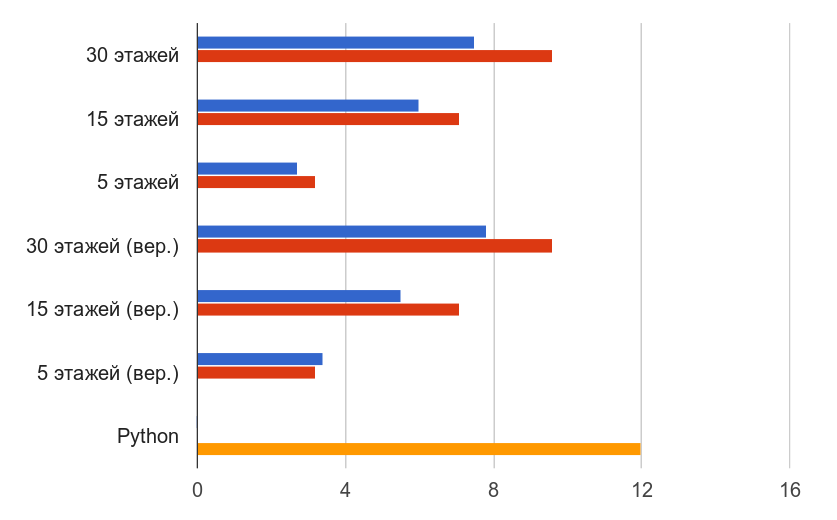
\includegraphics[width=180mm]{src/pictures/projectp1.png}
			\caption{Сравнение по среднему времени ожидания}\label{pt1}
		\end{figure}

		Более того, продвинутое решение требует небольшого улучшения, которое позволит с лёгкостью пройти тест на
			небольшом количестве этажей. Улучшение будет собой представлять не большое правило, которое бы могло увеличить
			глубину обхода дерева вариантов решений.
			
		Но не стоит забывать, что чем сложнее требуемый логический вывод, тем больше ресурсов необходимо системе для
			функционирования. Поэтому необходимо обратить внимание на диаграмму, которая представлена на рисунке \ref{pt2}.

		\begin{figure}[h]
			\centering
			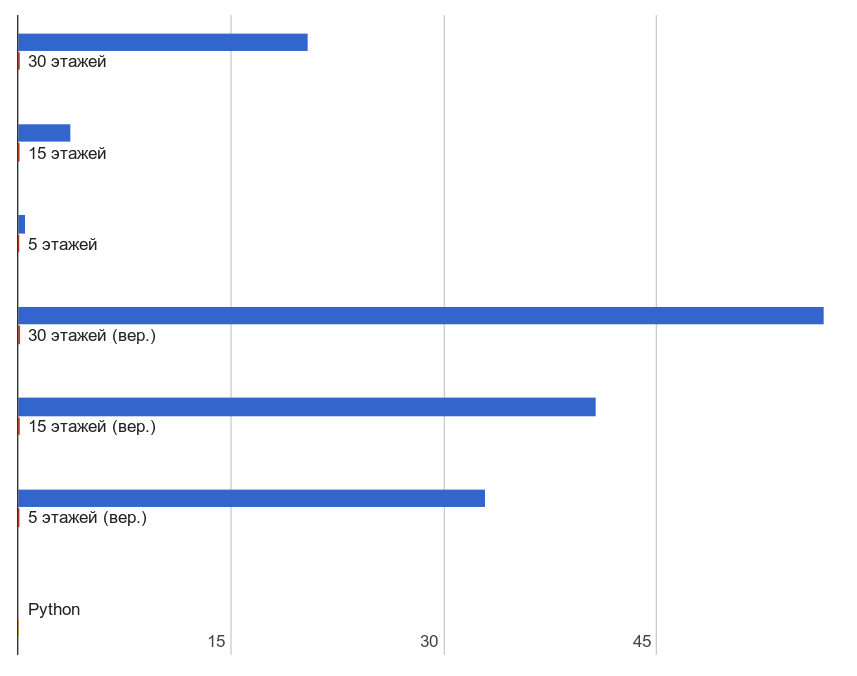
\includegraphics[width=180mm]{src/pictures/projectp2.png}
			\caption{Сравнение по времени выполнения}\label{pt2}
		\end{figure}

		Из диаграммы видно, что время, которое затрачено на построение логического вывода достаточно велико.
			Это показывает, что для своевременного решения необходимо достаточно большое количество ресурсов.
			Несмотря на тот факт, что на стройка разработанного программного обеспечения не будет занимать
			длительное время, что делает продукт более дешёвым, поддержание данной системы становится
			дорогостоящим процессом, за счёт потребности в дорогостоящем оборудовании.

		Исходя из этого имеется необходимость заняться оптимизацией данного программного решения,
			которое позволит снизить потребность в большом объёме ресурсов.

		И тем не менее, в наше время высокопроизводительное оборудование быстро удешевляется, развивается и
			становится более доступным. Более того, для мест со сложной инфраструктурой затраты на
			разработанное программное решение будет вполне целесообразным.

		Важно подчеркнуть ещё тот, что данное программная реализация является решением двух задач: моделирование 
			среды и построение логического вывода. А это значит, что если выделить блок отвечающий
			за моделирование среды и реализовать его на оптимизированном движке, то сразу будет
			получен большой прирост прирост в производительности.

		Таким образом, разработав данное программное решение, была получена платформа для разработки
			новых программных решений. Где можно будет выделить у данной системы два блока, с которыми
			будет возможно вести независимую разработку. Это позволит ускорить процесс развития данной системы
			и появится возможность заменять эти блоки на более сложные решения.
